\chapter{Visão geral}
\section{Nome do Jogo}
Ogof e o templo das joias.

\section{\textit{High Concept} do Jogo}

Lorem ipsul dolort sit amet consetur
\section{Gênero}
Fantasia

\section{Púbico Alvo}

Adolescentes entre 16 e 20 anos

\section{\textit{Game Flow}}

Lorem ipsul dolort sit amet consetur

\section{Estilo estético}

Lorem ipsul dolort sit amet consetur

\section{Inspirações}

\subsection{Outlander}
\subsection{Filha de Feiticeira}
\subsection{Desencanto}
\subsection{Os Vingadores - Guerra ininita}
\subsection{Franquia God of War}
\subsection{Sonhos de uma noite de verão}
\subsection{Brownies}
\subsection{Alux}

\section{Equipe de Desenvolvimento}

A equipe dividiu-se de forma a otimizar as forças de cada um dos integrantes, desta forma ficamos com a seguinte divisão de tarefas não rigidas. 

Marina atuou fortemente com o game design, character design e história. 

Pedro atuou como desenvolvedor e 

Eric atuou como arte técnica, animação e desenvolvimento

\chapter{Gameplay e Mecânicas}
\section{\textit{Gameplay}}

Durante as três primeiras fases, o jogador é apresentado a um dos personagens em seu ambiente natural, este é o momento para que se aprenda as diversas habilidades dos diferentes personagens.

As habilidade serão apresentadas ao jogador gradualmente, sem que o mesmo fique sobrecarregado de informações, ao mesmo passo que a dificuldade de inimigos também aumentará, objetivando manter o \textit{flow} do jogo.
\begin{citacao}
Segundo Myhaly inserir a definição de flow! \cite[74]{mihalyi2009}
\end{citacao}

Ao final das duas primeiras fases, o jogador iniciara uma nova fase com um novo personagem, já no  final da terceira, ele será levado também a uma nova fase, porém agora ele deverá controlar os três personagens de maneira cooperativa, para que unindo suas habilidades únicas progrida no jogo.


\section{Progressão do Jogo}

A progressão do jogo segue a linha de: o jogador precisa jogar individualmente pelo mundo dos três personagens (Duende, Xamã e Bruxa) para se adequar com as mecânicas de cada um e atingir um portal. Esse portal os levará para um HUB, onde os três personagens irão se encontrar e se unir como uma equipe para alcançarem seus objetivos. Caberá ao jogador de, durante o prosseguimento das fases, controlar e fazer uso das habilidades especiais dos personagens, um a um, para alcançar o inimigo chefe Ogof e o derrotar.

\section{Estrutura de Missões/Desafios}

A estrutura de missões segue sempre a mesma linha de pensamento de apresentar ao jogador um ambiente com objetos espalhados que deverão ser dispostos em pontos específicos dos cenários. Cabe ao jogador saber como e onde aplicar esses itens fazendo uso das habilidades específicas de cada personagem.

\section{Objetivos}

Segundo Jeremy Gibson, em seu livro \textit{"Introduction to Game Design, Prototyping and Development"}, por mais que todo jogo contenha um objetivo simples, finalizar e/ou ganhar o jogo, o jogador está a todo momento analisando diversos objetivos durante o processo. Gibson ainda divide esses objetivos em curto, médio e longo prazo. \cite{gibson2014}

Em Ogof e O Templo das Joias os objetivos de curto prazo são sobreviver aos diferentes combates e desafios para avançar no jogo. Como objetivo de médio prazo, o jogador não quer perder o rastro deixado pelo antagonista, e assim achar quem lhe foi tirado. Por fim, o objetivo de longo prazo é impedir que Ogof cumpra o ritual.

\section{Mecânicas}

Os personagens podem movimentar-se livremente pelo cenário, como descrito na sessão 2.6 Movimentação / Física. Além disso os personagens têm habilidades específicas, e como são de ambientes e tempos diferentes, percebem o cenário a sua volta de forma única. Isto é, alguns elementos podem ser vistos apenas por um dos personagens, e serão elementos chave para a progressão do jogo.

Abaixo está descrito, personagem a personagem, quais serão suas habilidades únicas. Estas terão cada uma sua barra de energia, e quando ativadas, consumirão desta energia.

\subsection{Duende}
\subsubsection{Crescer plantas}
Inspirado nas lendas dos Alux, que conseguem controlar os ventos e as chuvas, será possível crescer plantas em qualquer lugar, contanto que haja um substrato para a planta crescer, isto é,  madeira, solo ou água. Locais com pedras ou muito secos não permitirão que plantas se germinem.

Estas plantas serão utilizadas como plataformas para acessar áreas que precisem de uma plataforma ou ``elevador'' para serem acessadas.

Para ativar essa habilidade, utilizar-se-á o botão de habilidade 1 (vide 5.2 Sistema de Controle), e ao ativá-la será consumido sua ``energia de chuva''. Caso essa energia se esgote, não será possível ativar esta habilidade. Para recuperar esta energia ele deverá recolher fragmentos.


\subsubsection{Destruir plantas}
Esta habilidade deriva da habilidade anterior, mas irá destruir plantas existentes, ou mesmo plantas que foram criadas por "Crescer Plantas". Para ativá-la, deve-se utilizar o botão de habilidade 2 (Vide 5.2 Sistema de controle). Esta  habilidade consumirá do mesmo recurso que sua habilidade anterior. 


\subsubsection{Invisibilidade}
Inspirado em os ``duendes'' serem dificilmente vistos em diversas lendas, esta habilidade deixará o personagem invisível para os inimigos por um certo tempo, assim como as habilidades anteriores, ela terá uma barra de energia, que será consumida enquanto estiver invisível. Para recuperar a energia de invisibilidade, deverá coletar fragmentos.

Esta habilidade está mapeada para o botão de habilidade 3 



\subsection{Xamã}
\subsubsection{Curar}
Inspirado nos curandeiros das culturas Nativo-Americanas, em especial nos Pueblo, e nas tribos que acredita-se que tenham ancestralidade Pueblo, esta habilidade irá curar uma porcentagem da vida do objeto alvo, seja ele aliado, inimigo ou outro ser com vida.

Para utilizar essa habilidade será utilizado o botão de habilidade 1

\subsubsection{Habilidade 2}

\subsubsection{Olhos de águia}

O Xamã poderá evocar uma águia, para que possa visualizar dor outra perspectiva o ambiente em que se está. Ao ativar essa habilidade o jogador terá alguns segundos para controlar a águia, com uma mecânica de voo. Após esse tempo, a câmera do jogo voltará a focar no Xamã.

Além de voar, a Águia tem a vantagem de ser mais rápida que os personagens e não chamar a atenção de inimigos.

Esta habilidade não tem barra de energia a ser consumida, mas não poderá ser utilizada quando em combate, e será ativada com o botão de habilidade 3. 


\subsection{Bruxa}

\subsubsection{Habilidade 1}

\subsubsection{Habilidade 2}

\subsubsection{Habilidade 3}


\subsection{Ataques}
Em conjunto com as habilidades, cada personagem terá dois ataques, um com o botão direito do mouse e outro com o botão esquerdo do mouse. 


\section{Movimentação / Física}
A movimentação dentro do jogo se dará utilizando as teclas W, A, S, e D do teclado, por ser um padrão já conhecido e utilizado em muitos jogos.

Com o movimento do mouse, o jogador conseguirá rotacionar a câmera do jogo para ter uma melhor visibilidade do cenário, e assim, maiores chances de resolver os desafios.

Para tal, será utilizado o motor de física fornecido pela própria engine Unity3D.

Para maiores detalhes consulte a sessão 5.2 - Sistema de Controle deste documento.

\section{Objetos}

TODO:

\section{Ações}
O jogador poderá se movimentar livremente pelo cenário, bem como atacar, pular, interagir, coletar e utilizar as habilidades específicas de cada um dos personagens.

Para maiores detalhes do uso de tais ações, verifique a sessão 5.2 Sistemas de Controle.

\section{Combate}
O combate irá ganhar dificuldade de forma gradual enquanto o jogador avança pelo jogo, com diferentes criaturas de diferentes níveis de poder e tipos de ataque (corpo a corpo e à distancia, por exemplo), e pontos de vida. 

Para manter a sensação de urgência ao jogador e fornecer um melhor sistema de combate, utiliza-se um comportamento de inteligência artificial conhecido como círculo de batalha, presente em diversos jogos como God of War, Dark Souls, Okami e outros \cite{BattleCi}.

Para maiores detalhes leia a sessão 6.1 - Oponentes e IA Inimiga

\section{Economia}

Não há economia planejada para o jogo.

\section{Opções do Jogo}

Segundo o livro Design e Desenvolvimento de Jogos, uma das formas de se identificar jogadores é classificá-los como \textit{hardcore}, que são jogadores experientes que gostam de ser desafiados, e casuais, que são jogadores que preferem jogos mais fáceis e costumeiramente abandonam jogos que são demasiadamente desafiadores \cite{pradadesign}. 

O livro ainda indica que para atingir ambos os públicos é interessante que se tenha ao menos dois níveis de dificuldades em um jogo. Assim, Ogof e O Templo das Joias contará com variados níveis de dificuldade, que afetarão como a IA inimiga irá se comportar, bem como pontos de vida e ataque.

Será possível também ativar e desativar legendas para as partes de histórias e diálogos no jogo. E por fim o jogador poderá selecionar a resolução do jogo que prefere jogar.

\section{Salvar \& Replay}

O jogo contém um sistema de auto-salvamento, que será ativado em certos momentos chave do jogo. Além disso será possível salvar pelo menu de pause do jogo, para retornar futuramente no estado em que parou.

\section{Easter Eggs, Cheats, bônus}

No momento não estão sendo planejados Easter Eggs ou Cheats, contudo durante o jogo alguns objetos coletáveis darão acesso às artes conceituais do jogo.


\chapter{Arte do Game}

\section{Elementos Visuais}

Descreva os elementos chave; como estão sendo desenvolvidos; qual o estilo. Inclua detalhes sobre a direção de arte, paleta de cores e inspirações.

\subsection{Inspirações}
Todos os personagens foram baseados em estatuetas artesanais, desenhados em 2D e por fim modelados em 3D. 
\subsection{Duende}
\begin{figure}[htb]
	\caption{\label{duendeRef}duendeRef}
	\begin{center}
	    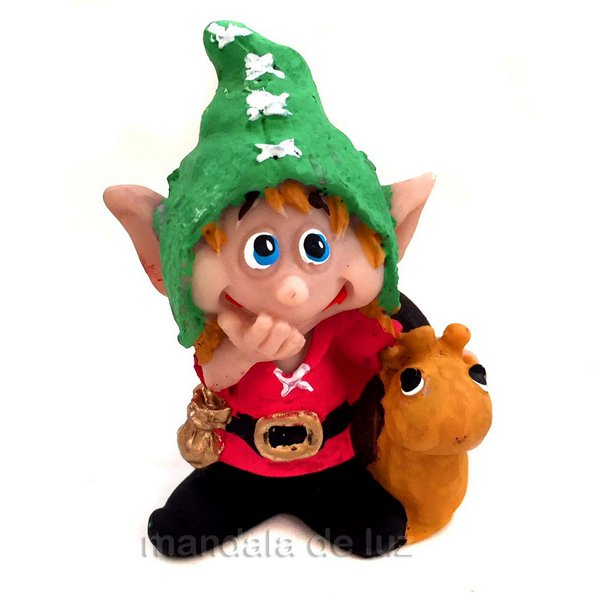
\includegraphics[width=\textwidth]{imagens/duendeRef.jpg}
	\end{center}
	\legend{Fonte: Mandala de Luz - https://www.mandaladeluz.com.br/pumy-duende-amigo-chapeu-verde-8cm}
\end{figure}



\begin{figure}[htb]
	\caption{\label{duendePos}duendePos}
	\begin{center}
	    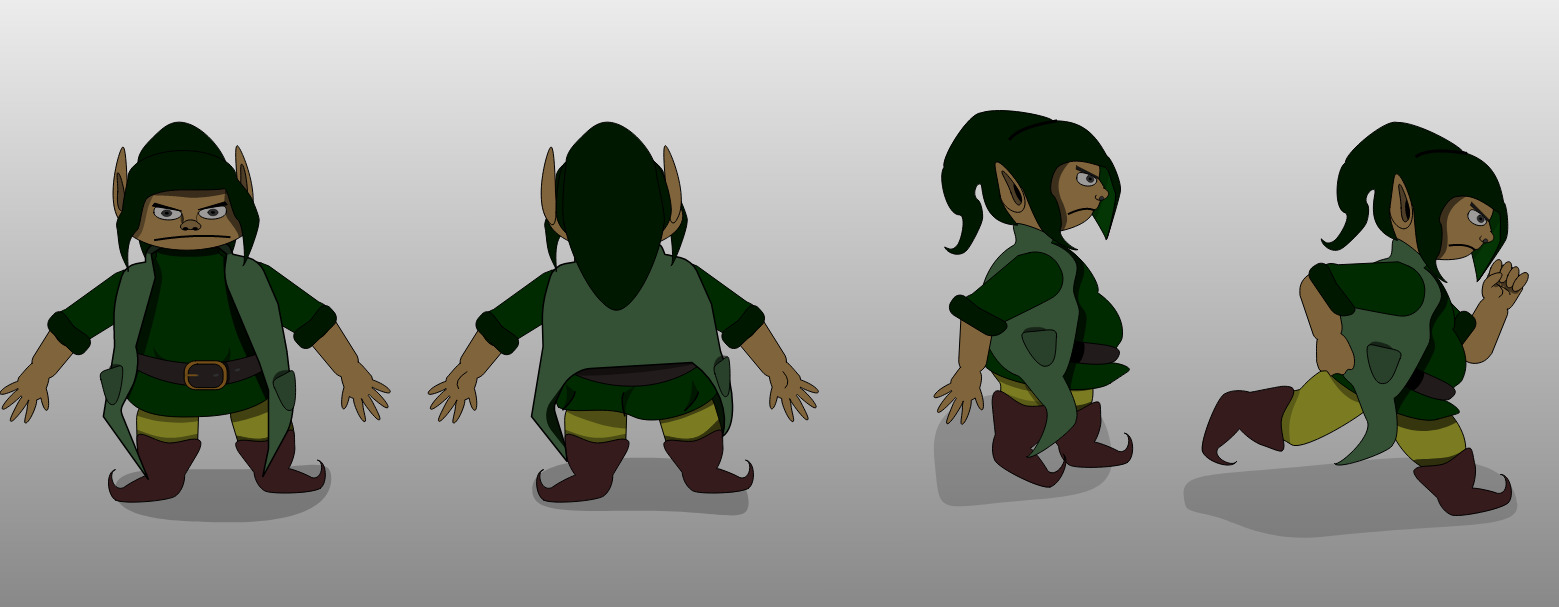
\includegraphics[width=\textwidth]{imagens/duendePosições.jpeg}
	\end{center}
	\legend{Fonte: Autoria Própria - Marina Araujo}
\end{figure}



\subsection{Ogof}
\begin{figure}[htb]
	\caption{\label{mago}mago}
	\begin{center}
	    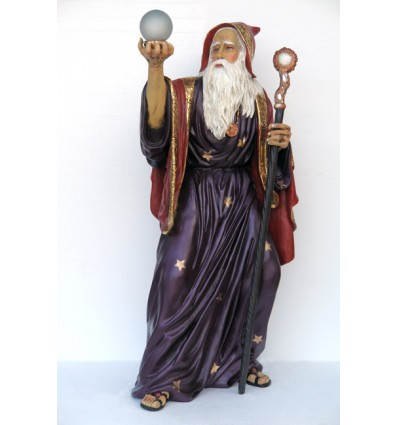
\includegraphics[width=\textwidth/2]{imagens/mago.jpg}
	\end{center}
	\legend{Fonte: Macocaya - https://macocaya.es/es/varios/3134-mago-con-bola.html}
\end{figure}

\begin{figure}[htb]
	\caption{\label{Ogof}Ogof}
	\begin{center}
	    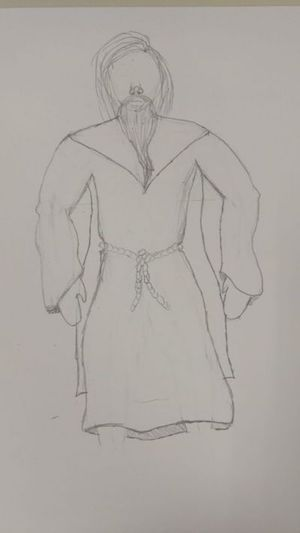
\includegraphics[width=\textwidth/2]{imagens/Ogof.jpg}
	\end{center}
	\legend{Fonte: Autoria Própria - Marina Araujo}
\end{figure}

\subsection{Paleta de cores}
\begin{figure}[htb]
	\caption{\label{paleta}paleta}
	\begin{center}
	    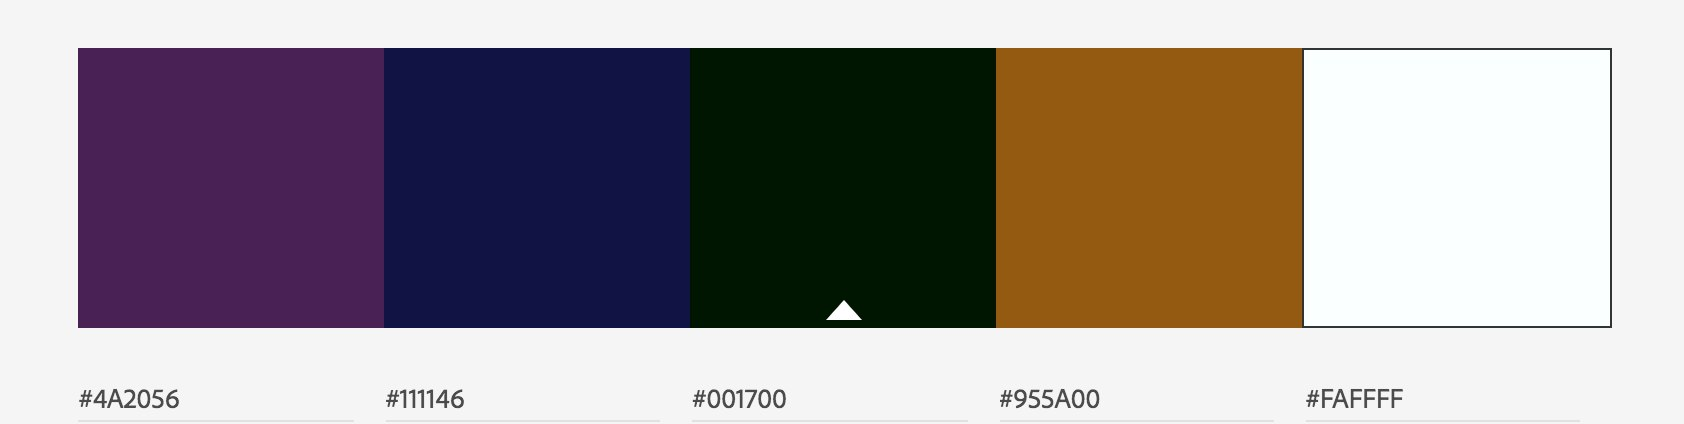
\includegraphics[width=\textwidth/2]{imagens/paleta.jpg}
	\end{center}
	\legend{Fonte: Própria Autoria}
\end{figure}

\section{Elementos Sonoros}

Descreva os elementos chave; como estão sendo desenvolvidos; qual o estilo musical. Inclua detalhes sobre efeitos sonoros e inspirações.

\chapter{Narrativa, Ambientação e Personagens}

\section{História e Narrativa}

Descreva os elementos chave; como estão sendo desenvolvidos; qual o estilo musical. Inclua detalhes sobre efeitos sonoros e inspirações.

\section{Mundo do Jogo}

Descreva e apresente o mundo geral do jogo, inclusive com a apresentação visual.

\section{Áreas do Jogo}

Descreva e apresente o mundo geral do jogo, inclusive com a apresentação visual.


\section{Personagens}

\subsection{Ogof}
\subsection{Duende}
\subsection{Bruxa}
\subsection{Xamã}

Lorem ipsul dolort sit amet consetur

\section{Fases}

Descreva cada fase incluindo sinopse, objetivos e detalhes dos acontecimentos que se desenrolam em seu percurso.


\section{Fase de Treino e/ou Tutorial}

Descreva como funciona a fase de treino ou o tutorial do jogo que aparece na tela.


\chapter{Interface}

\section{Sistema Visual}

Lorem ipsul dolort sit amet consetur


\section{Sistema de Controle}

Lorem ipsul dolort sit amet consetur

\section{Sistema de Ajuda}

Lorem ipsul dolort sit amet consetur

\chapter{Inteligência Artificial (AI)}
Esta sessão será preenchida no próximo semestre.

\section{Oponentes e AI Inimiga}

Para os oponentes pretende-se utilizar a técnica de Circulo de batalha explicada pelo \citeonline{BattleCi} em seu artigo. No próximo semestre preencheremos esta sessão com maiores informações e explicações de suas aplicações.


\section{AI parceira ou não-inimigas}


\section{AI de Suporte}


\chapter{Aspectos Técnicos}

\section{Plataforma de Produção}

Lorem ipsul dolort sit amet consetur

\section{Hardware e Software de Desenvolvimento}

Lorem ipsul dolort sit amet consetur

\section{Requerimentos de Rede}


\chapter{Cronograma}

\section{Cenário Atual}

Foram bem definidas as histórias e mecânicas de 2 dos três personagem jogáveis, bem como a motivação do antagonista.

Conseguiu-se definir as grandes áreas do jogo e suas inspirações, e desafios pontuais que os personagens encontrarão.

\section{Próximos Passos}

Para os próximos passos do projeto, será feito uma lapidação e maior definição das características e habilidades da personagem Bruxa.

Será iniciada a parte técnica de execução do projeto, inciciando-se pela modelagem 3D Low Poly dos personagens. Espera-se que seja empenhada 2 semanas para cada personagem, bem como sua animação, com um dos personagens em mão será iniciada a implementação de mêcanicas e a programação nescessária.

A partir da segunda semana de implementação das mecânicas serão feitas rodadas de testes e feedbacks com \textit{beta testers} quinzenalmente, para polimento e avaliação de diversão.


\section{Cronograma}


\chapter{Modelo de Negócio}
Esta sessão será desenvolvida futuramente.
% Descreva nessa seção como pretende monetizar o jogo, se é que haverá monetização. Se for vendido, por exemplo, informe qual a faixa de preço. Se houver compras dentro do jogo, como serão feitas? Quais serão as estratégias de divulgação para ampliar a comunidade de fãs e possíveis compradores (redes sociais, mídia especializada, demo, early access etc.).
% Mesmo que não haja monetização no seu jogo, nesta seção devem ser descritos os elementos definidos pelo(a) orientador(a) responsável pela disciplina Empreendedorismo, sendo neste momento o canvas comentado e a análise SWOT do jogo.


